\begin{frame}
\frametitle{Cyclus}
\begin{block}{What is Cyclus?}
	Cyclus is a modular agent based fuel cycle simulator for tracking commodity transactions
	between facilities.
\end{block}
\begin{figure}
	\centering
	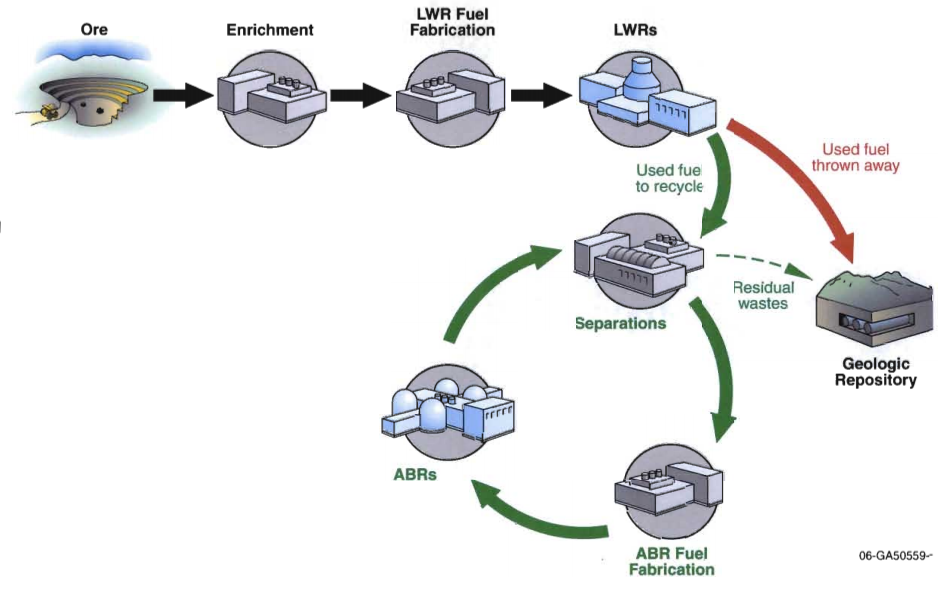
\includegraphics[width=0.7\linewidth]{./images/lanl-fuel-cycle.png}
	\label{fig:fuelcycle}
\end{figure}
\end{frame}

\begin{frame}
\frametitle{Why Cyclus?}
Cyclus allows the construction of specific scenarios through the addition of archetypes. These archetypes are
modular and the transactions can be tracked.
	\begin{figure}
		\centering
		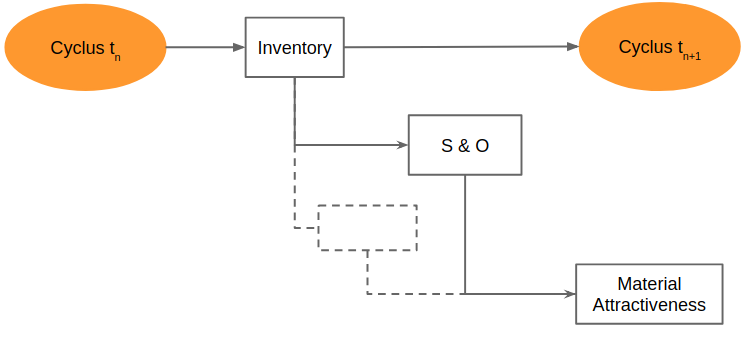
\includegraphics[width=0.9\linewidth]{./images/diversion1}
		\caption{Material transactions within Cyclus.}
		\label{fig:transactions}
	\end{figure}
\end{frame}